\section{组合图}
\label{sec:composite-plots}

SAC中与窗口有关的概念有三个,如图\ref{fig:window-viewspace-viewport}:
\begin{itemize}
\item windows:对于xwindows设备,window即图\ref{fig:plot}中的大小,其默认长宽比为
    11.0/8.5=1.294;对于sgf或者pdf和ps,可以认为window的大小即为A4纸张的大小。
\item viewspace:window内可以用于绘图的部分;
\item viewport:对于组合图,每个子图占据的空间;
\end{itemize}

\begin{figure}[H]
\centering
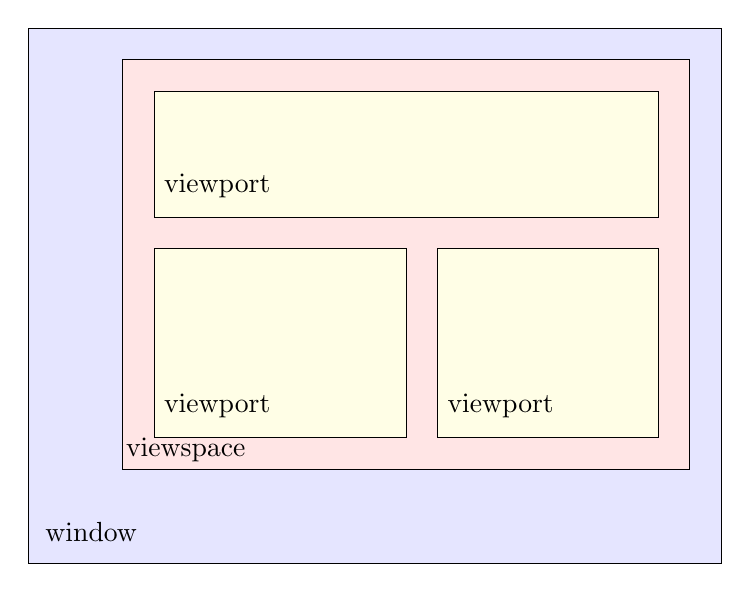
\begin{tikzpicture}[scale=0.8]
    \draw[fill=blue!10] (0,0) rectangle (11.0,8.5);
    \draw[fill=red!10] (1.5,1.5) rectangle (10.5,8);
    \draw[fill=yellow!10] (2,5.5) rectangle (10,7.5);
    \draw[fill=yellow!10] (2,2.0) rectangle (6,5.0);
    \draw[fill=yellow!10] (6.5,2.0) rectangle (10,5.0);
    \draw (1,0.5) node {window};
    \draw (2.5,1.8) node {viewspace};
    \draw (3.0,6) node {viewport};
    \draw (3.0,2.5) node {viewport};
    \draw (7.5,2.5) node {viewport};
\end{tikzpicture}
\caption{window、viewspace和viewport}
\label{fig:window-viewspace-viewport}
\end{figure}

默认情况下,在每个使用绘图命令时,整个绘图窗口会更新,所以每次都会显示不同的图像。
\nameref{cmd:beginframe}命令会关窗口的自动更新,因而可以用于绘制组合图。当然还有
\nameref{cmd:endframe}来重新启动窗口的自动更新。

\begin{SACCode}
SAC> fg seis                        // 生成数据
SAC> beginframe                     // 关闭自动更新
SAC> xvport 0.1 0.9                 // 设定X viewport
SAC> yvport 0.7 0.9                 // 设定Y viewport
SAC> title 'Seismic Trace'          // 设定标题
SAC> fileid off                     // 不显示文件id
SAC> qdp off                        // 关闭快速绘图
SAC> p                              
SAC> fft wmean                      // FFT
SAC> xvport .1 .45                  
SAC> yvport .15 .55
SAC> title 'Amplitude Response (linlog)'
SAC> ylim 1e-5 1                    // Y轴范围
SAC> psp am linlog                  // 绘制振幅谱(linlog)
SAC> xvport .55 .9                  
SAC> title 'Amplitude Response (loglog)'
SAC> xlim 1 60
SAC> psp am loglog                  // 绘制振幅谱(loglog)
SAC> endframe                       // 启动自动更新
\end{SACCode}

\begin{figure}[H]
\centering
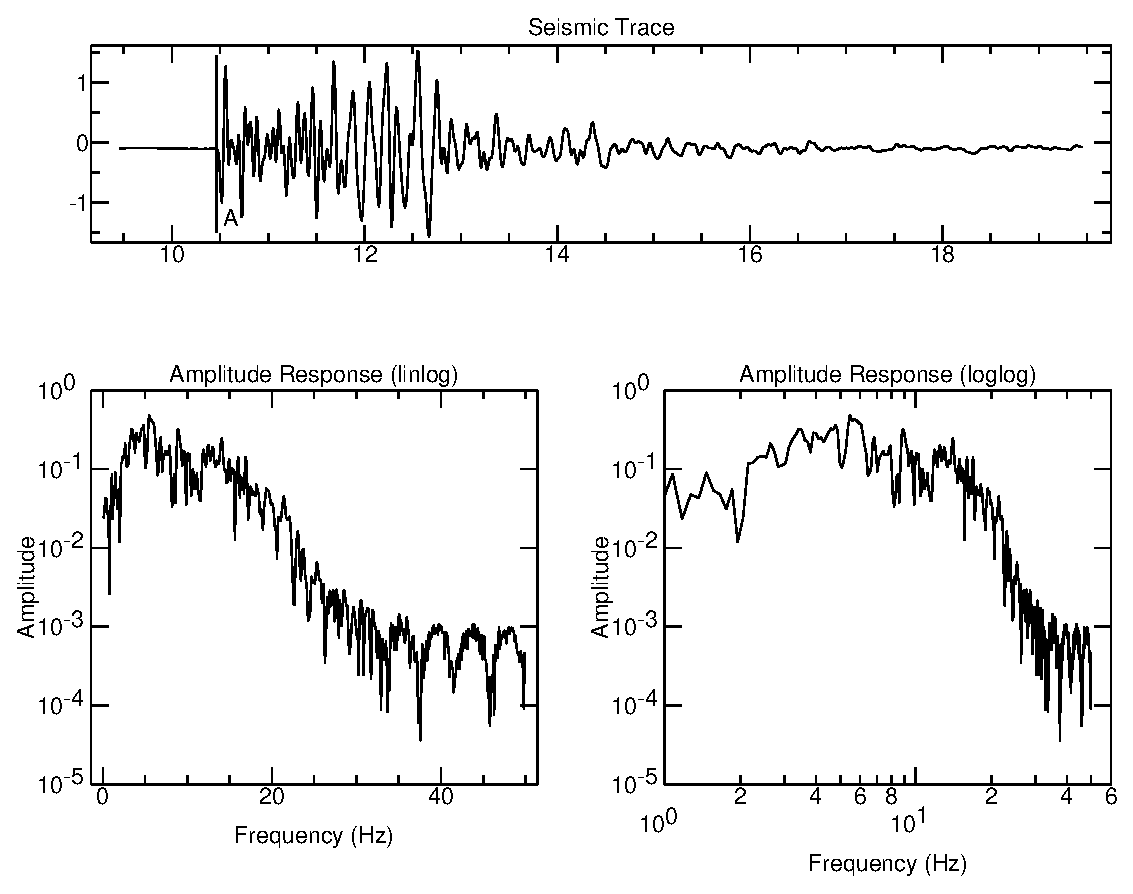
\includegraphics[width=0.8\textwidth]{composite-plot}
\caption{绘制组合图}
\label{fig:composite-plot}
\end{figure}
